\section{Thevenin Equivalent Circuits}
\label{thevenin_equivalence}

\textit{Thevenin's theorem} says that if you have a circuit with two outputs that includes any combination of voltage sources and resistors (actually \textit{current} sources too), then it is always functionally equivalent to a simpler circuit containing only one voltage source $V_{\rm Th}$ and one internal resistance $R_{\rm Th}$.  No electrical measurement can distinguish between the two. Thevenin's theorem makes it easier to figure out how a complicated circuit will interact with other circuits or components, for instance if a load resistance is connected to the output terminals of the circuit below.

\begin{center}
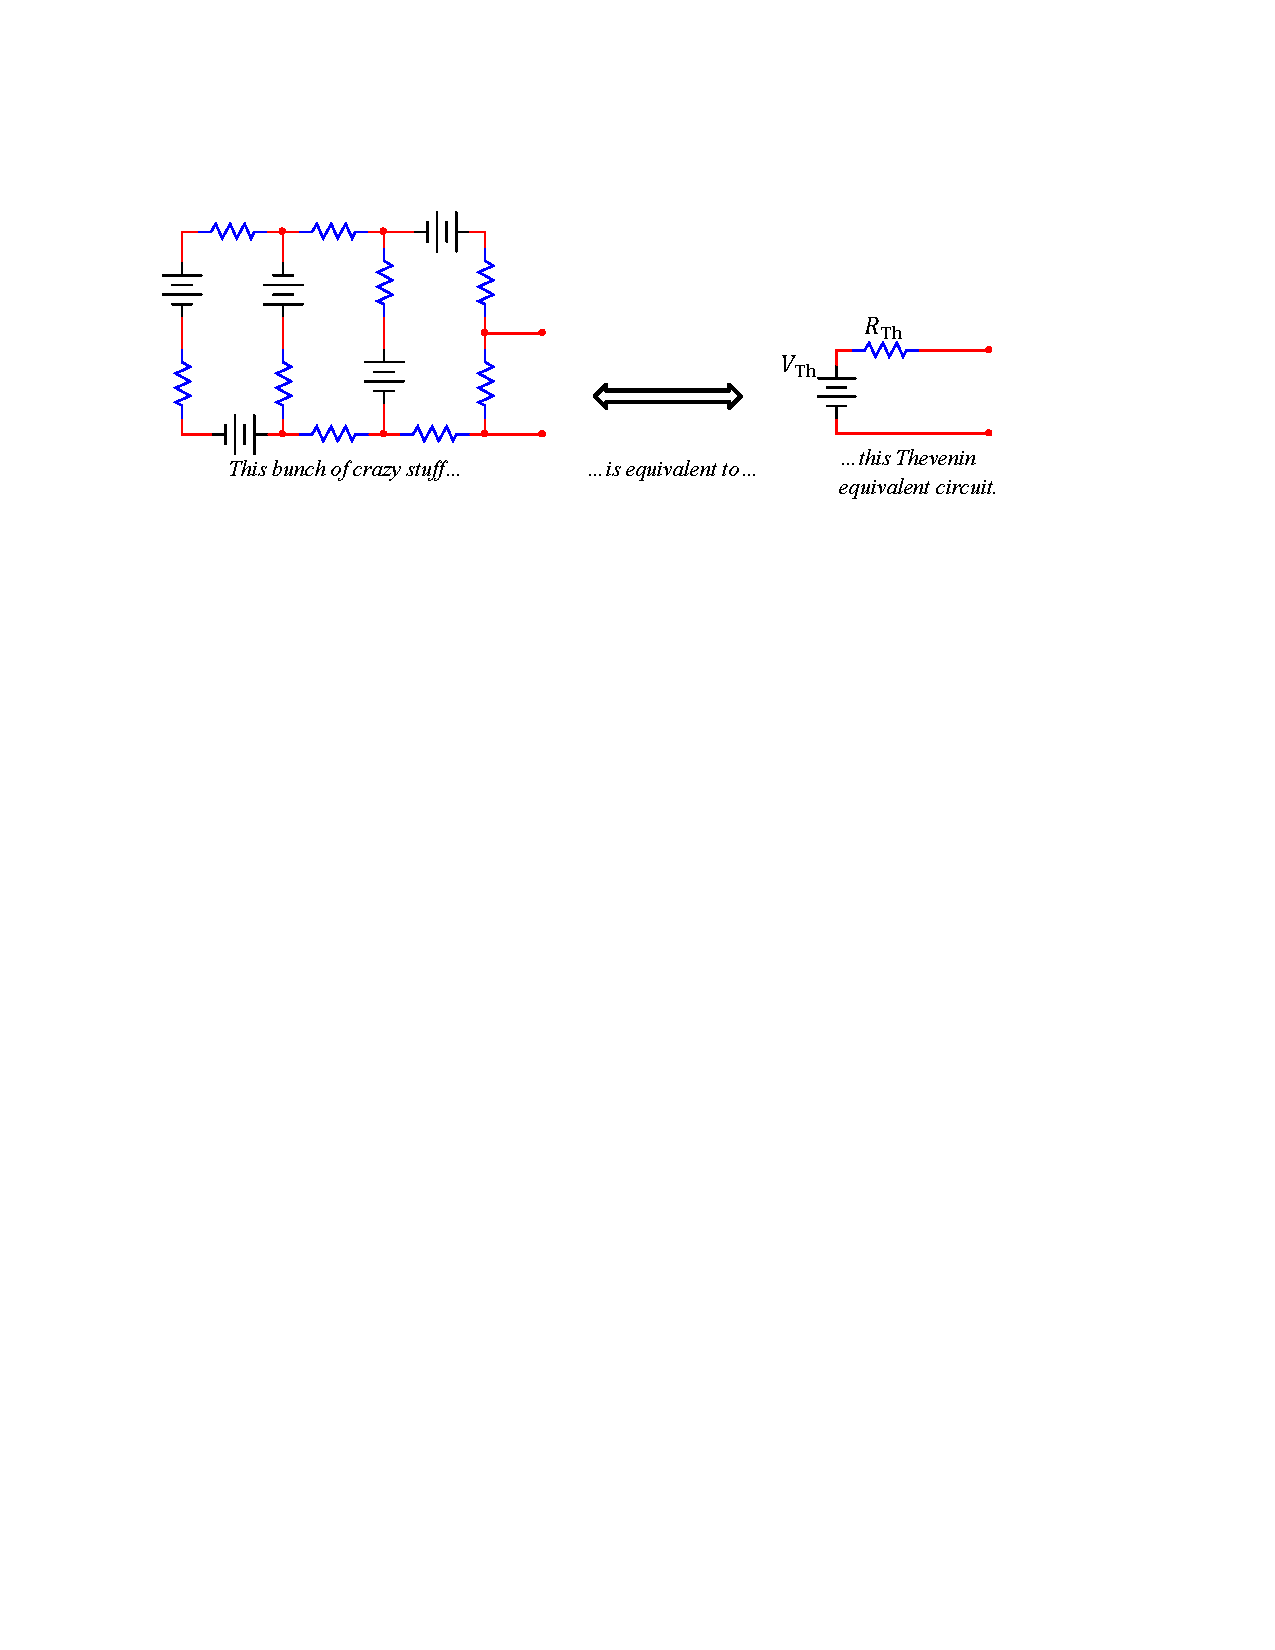
\includegraphics{appendices/thevenin_equivalence/thevenin_overview.pdf}
\end{center}

Here's how you find the values of $V_{\rm Th}$ and  $R_{\rm Th}$.
\begin{description}[labelindent=0.25in, leftmargin=0.5in]
\item[Step 1:] Find the open-circuit output voltage (the voltage with a very high load resistance).  This is  $V_{\rm Th}$, called the \textit{Thevenin equivalent voltage} or \textit{Thevenin voltage}. 

\item[Step 2:] Find the short-circuit output current $I_{\rm short}$ (the current with a very low load resistance).  The \textit{Thevenin equivalent resistance} is given by $R_{\rm Th}  = V_{\rm Th} / I_{\rm short}$.

\item[Step 2 (alternate):] Imagine shorting out all of the voltage sources, replacing any voltage source with a wire (and replacing any \textit{current} source with an open).  Then find the resistance between the output terminals (with no additional load resistance $R_{\rm load}$ connected); this is $R_{\rm Th}$.
\end{description}

\textbf{Example Problem}

For the circuit below, draw the Thevenin equivalent circuit and find values for $V_{\rm Th}$ and  $R_{\rm Th}$.

\begin{center}
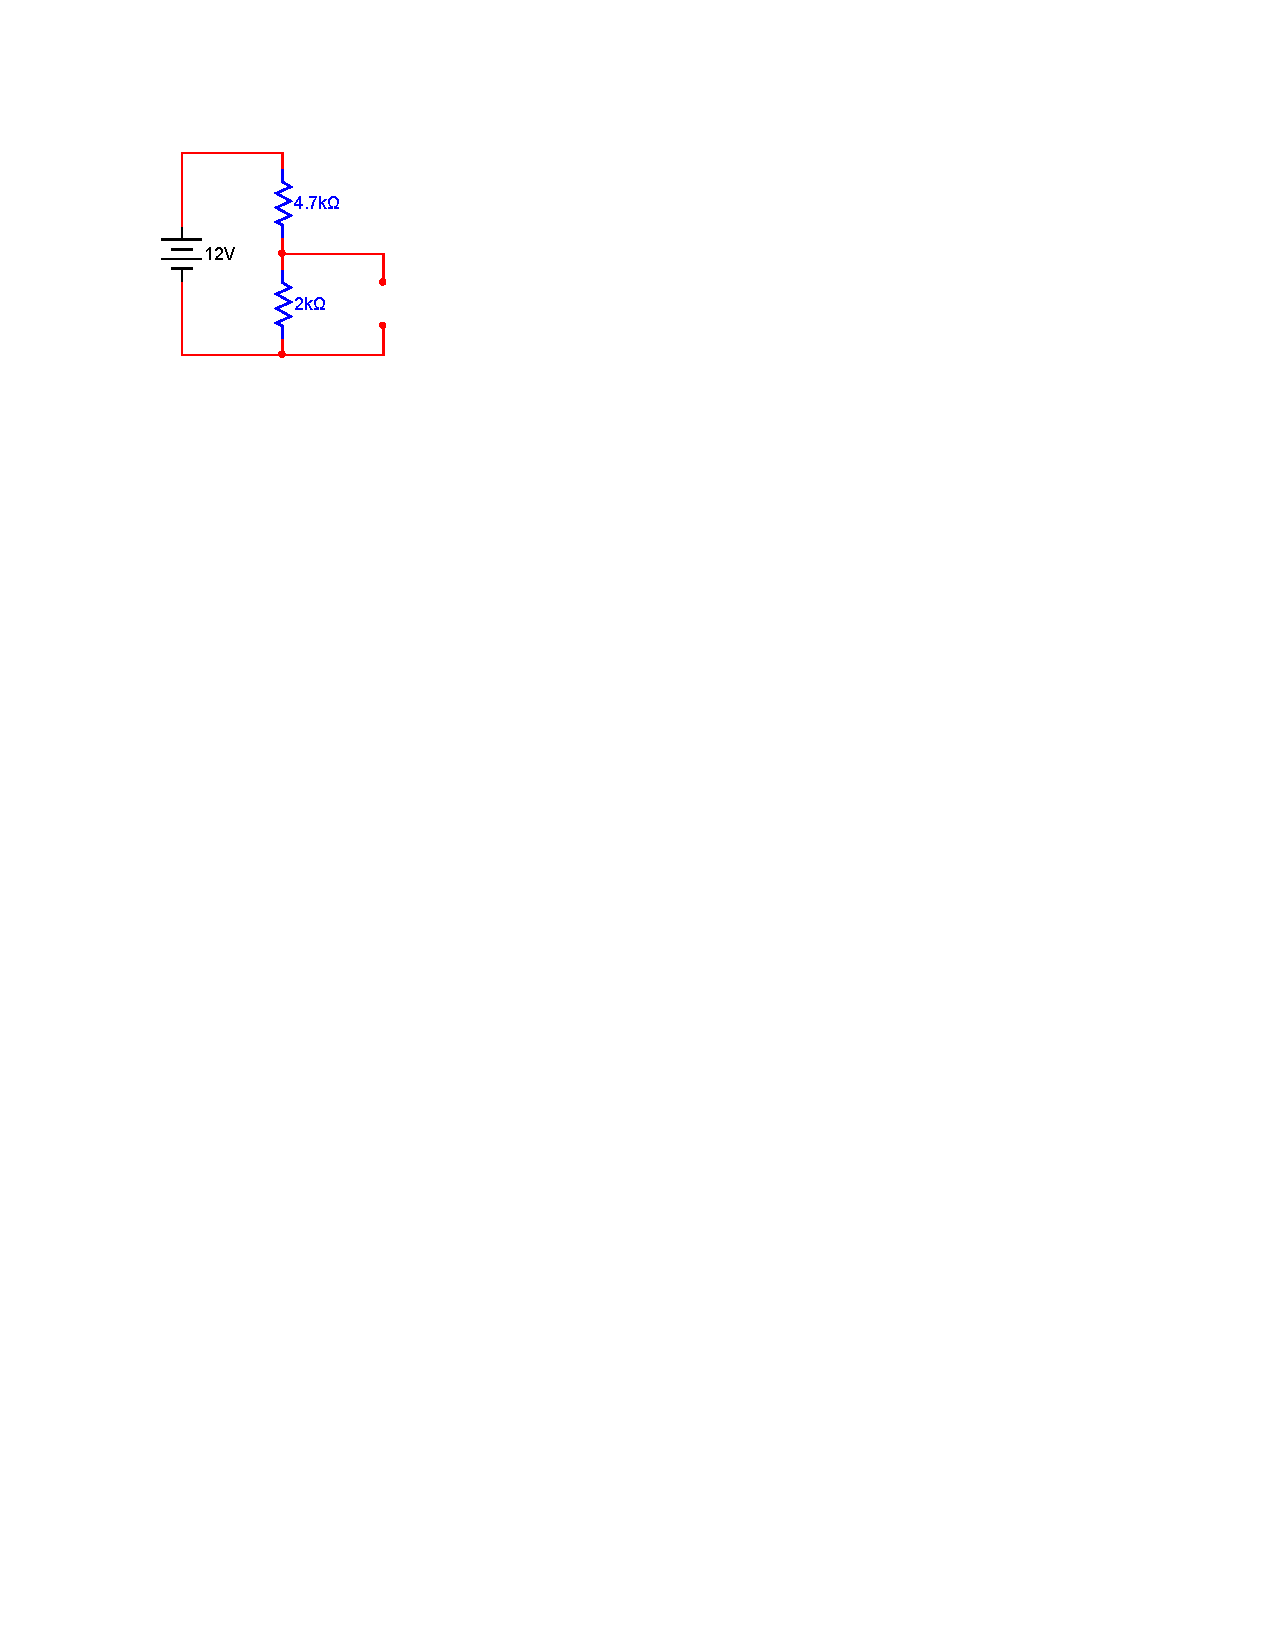
\includegraphics{appendices/thevenin_equivalence/thevenin_ex1.pdf}
\end{center}

\begin{description}[labelindent=0.25in, leftmargin=0.5in]
\item[Step 1:] What is the voltage across the output leads (across the $2\kohm$ resistor) with no load attached?  This is $V_{\rm Th}$.

\pagebreak[3]
\item[Step 2:] What is the current shown on the ammeter below?  So what is $R_{\rm Th}$?

\begin{center}
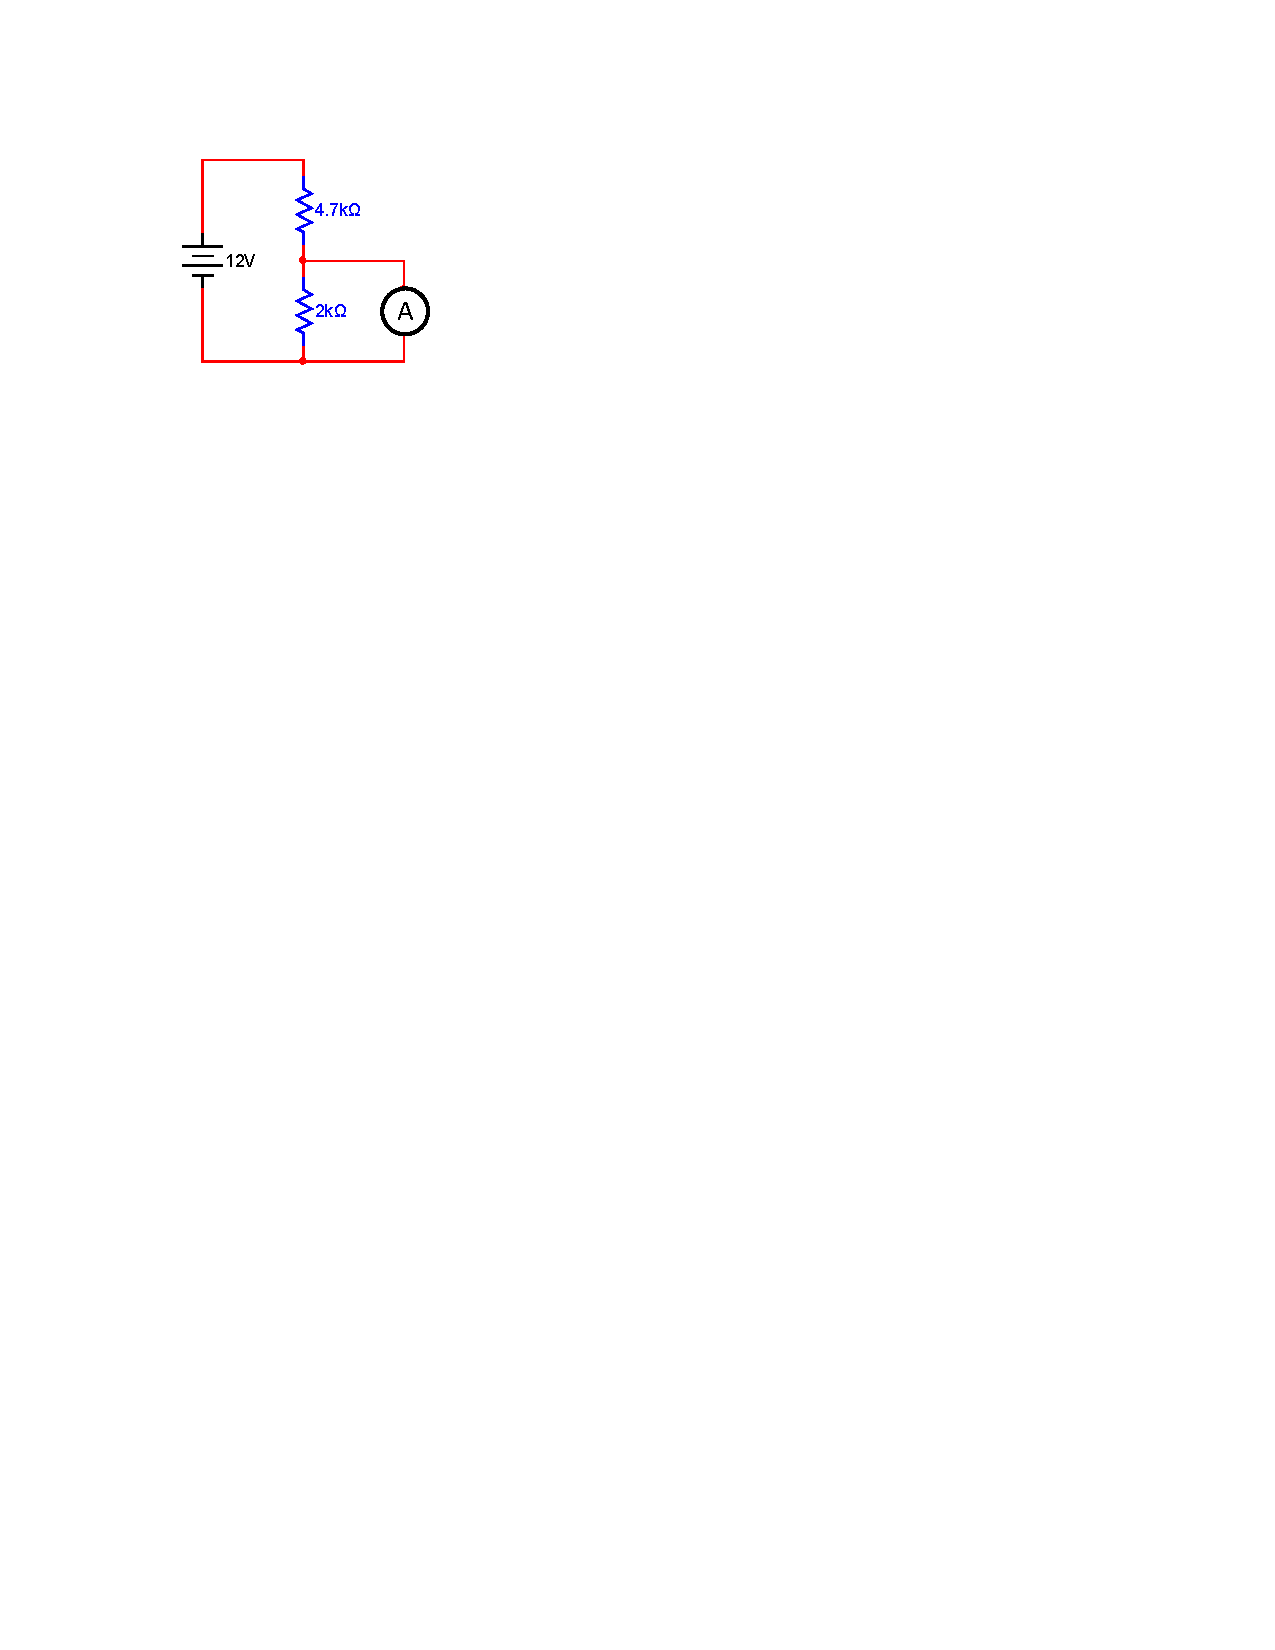
\includegraphics{appendices/thevenin_equivalence/thevenin_ex2.pdf}
\end{center}

\item[Step 2 (alternate):] With the voltage source short-circuited as in the picture below, what is the resistance between the two output leads?  

\begin{center}
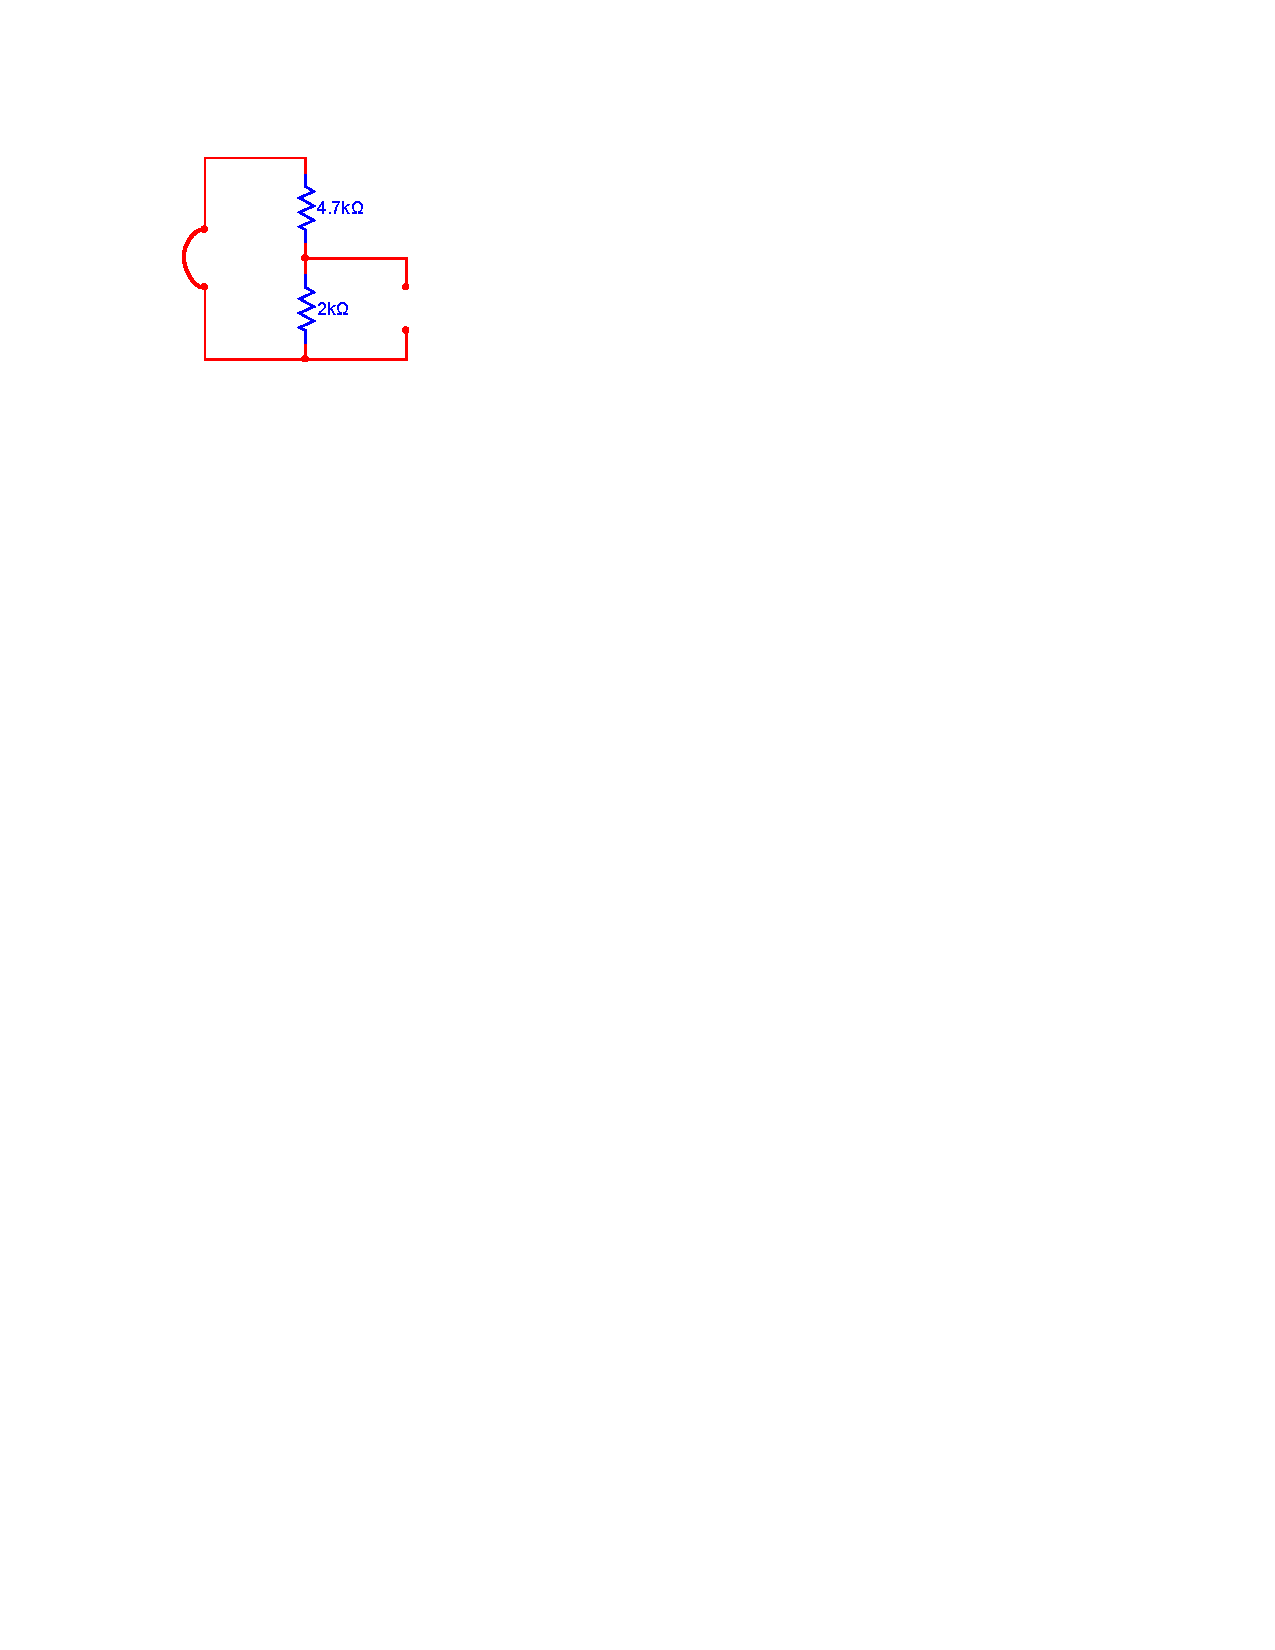
\includegraphics{appendices/thevenin_equivalence/thevenin_ex3.pdf}
\end{center}
\end{description}
\vfill
\hfill\textit{Answers:}  $V_{\rm Th}=3.58$ volts; $I_{\rm short}=2.55$ mA;  $R_{\rm Th} =1.40\kohm$. 

